\label{sec:result}
The result of the analysis can be seen in Figure \ref{fig:hitratio} - \ref{fig:hitratio-data} and Table \ref{tab:similarity}. Figure \ref{fig:hitratio} shows, for the different models and data types, the overall hit ratio of correct classification as a function of vocabulary size after $\chi^2$ pruning. By comparing the figures it can be noted that the maximum accuracy of 76\% is attained with binary inputs by \mn\ at a vocabulary size of 1022 words. Another observation is that \bn\ is sensitive to vocabulary size compared to other models and \svm\  seems in contrast to \bn\ more robust to changes in vocabulary size. More results derived from these figures are that \rf\ is independent of the feature format and \hy\ follows the behavior of \mn.
\\\\
The confusion matrices in Figure \ref{fig:confmat} describes the accuracy for specific topics. The rightmost column describes for a certain topic how many articles it contains and the accuracy of the topic. The bottom row describes for a certain predicted class, how many times that was the target class, and the accuracy when predicted. One can observe that Sports and Education are fairly easy to classify in contrast to Technology which is often misclassified as Science \& Environment. Notable is that \rf\ has a tendency of predicting Sports.
\\\\
Figure \ref{fig:hitratio-data} shows, for each model, how the hit rate depends on number of articles used as training set. For each selected subset of size 6 to 503 articles the 500 features with the highest $\chi^2$ scores are kept in the vocabulary and used to train the classifiers in order to keep the dimension of the feature space constant.
\\\\
In Table \ref{tab:similarity} a comparison of the similarity of prediction when mispredicting is shown. The values resembles, given that both classifiers predicted wrong class, how many times they predicted the same class.
%Table of similarities
\begin{table}[h]\footnotesize
	\caption{Percentage that two classifiers, when both classifying wrong, classifies test to the same class. A total of 231 articles were tested. A vocabulary size of 511 words and the data type \emph{"Mapped value from 0 to 1"} was used.}
	\begin{tabular}{r|cccc}
	\ 		 	& Bernoulli & Multin. 	&RF 		&SVM \\ \hline
	Bernoulli 	&100\%   	&67.3\%   	&69.0\%   	&58.8\%\\
	Multin. 	&67.3\%  	&100\%   	&78.6\%   	&76.9\%\\
	RF 			&69.0\%   	&78.6\%  	&100\%   	&75.4\%\\
	SVM 		&58.8\%   	&76.9\%   	&75.4\%  	&100\%
	\end{tabular}
	\label{tab:similarity}
\end{table}
\onecolumn
\newcommand{\figwidth}{0.49\textwidth}
\begin{figure}[H]
	\centering
	\begin{subfigure}[b]{\figwidth}
		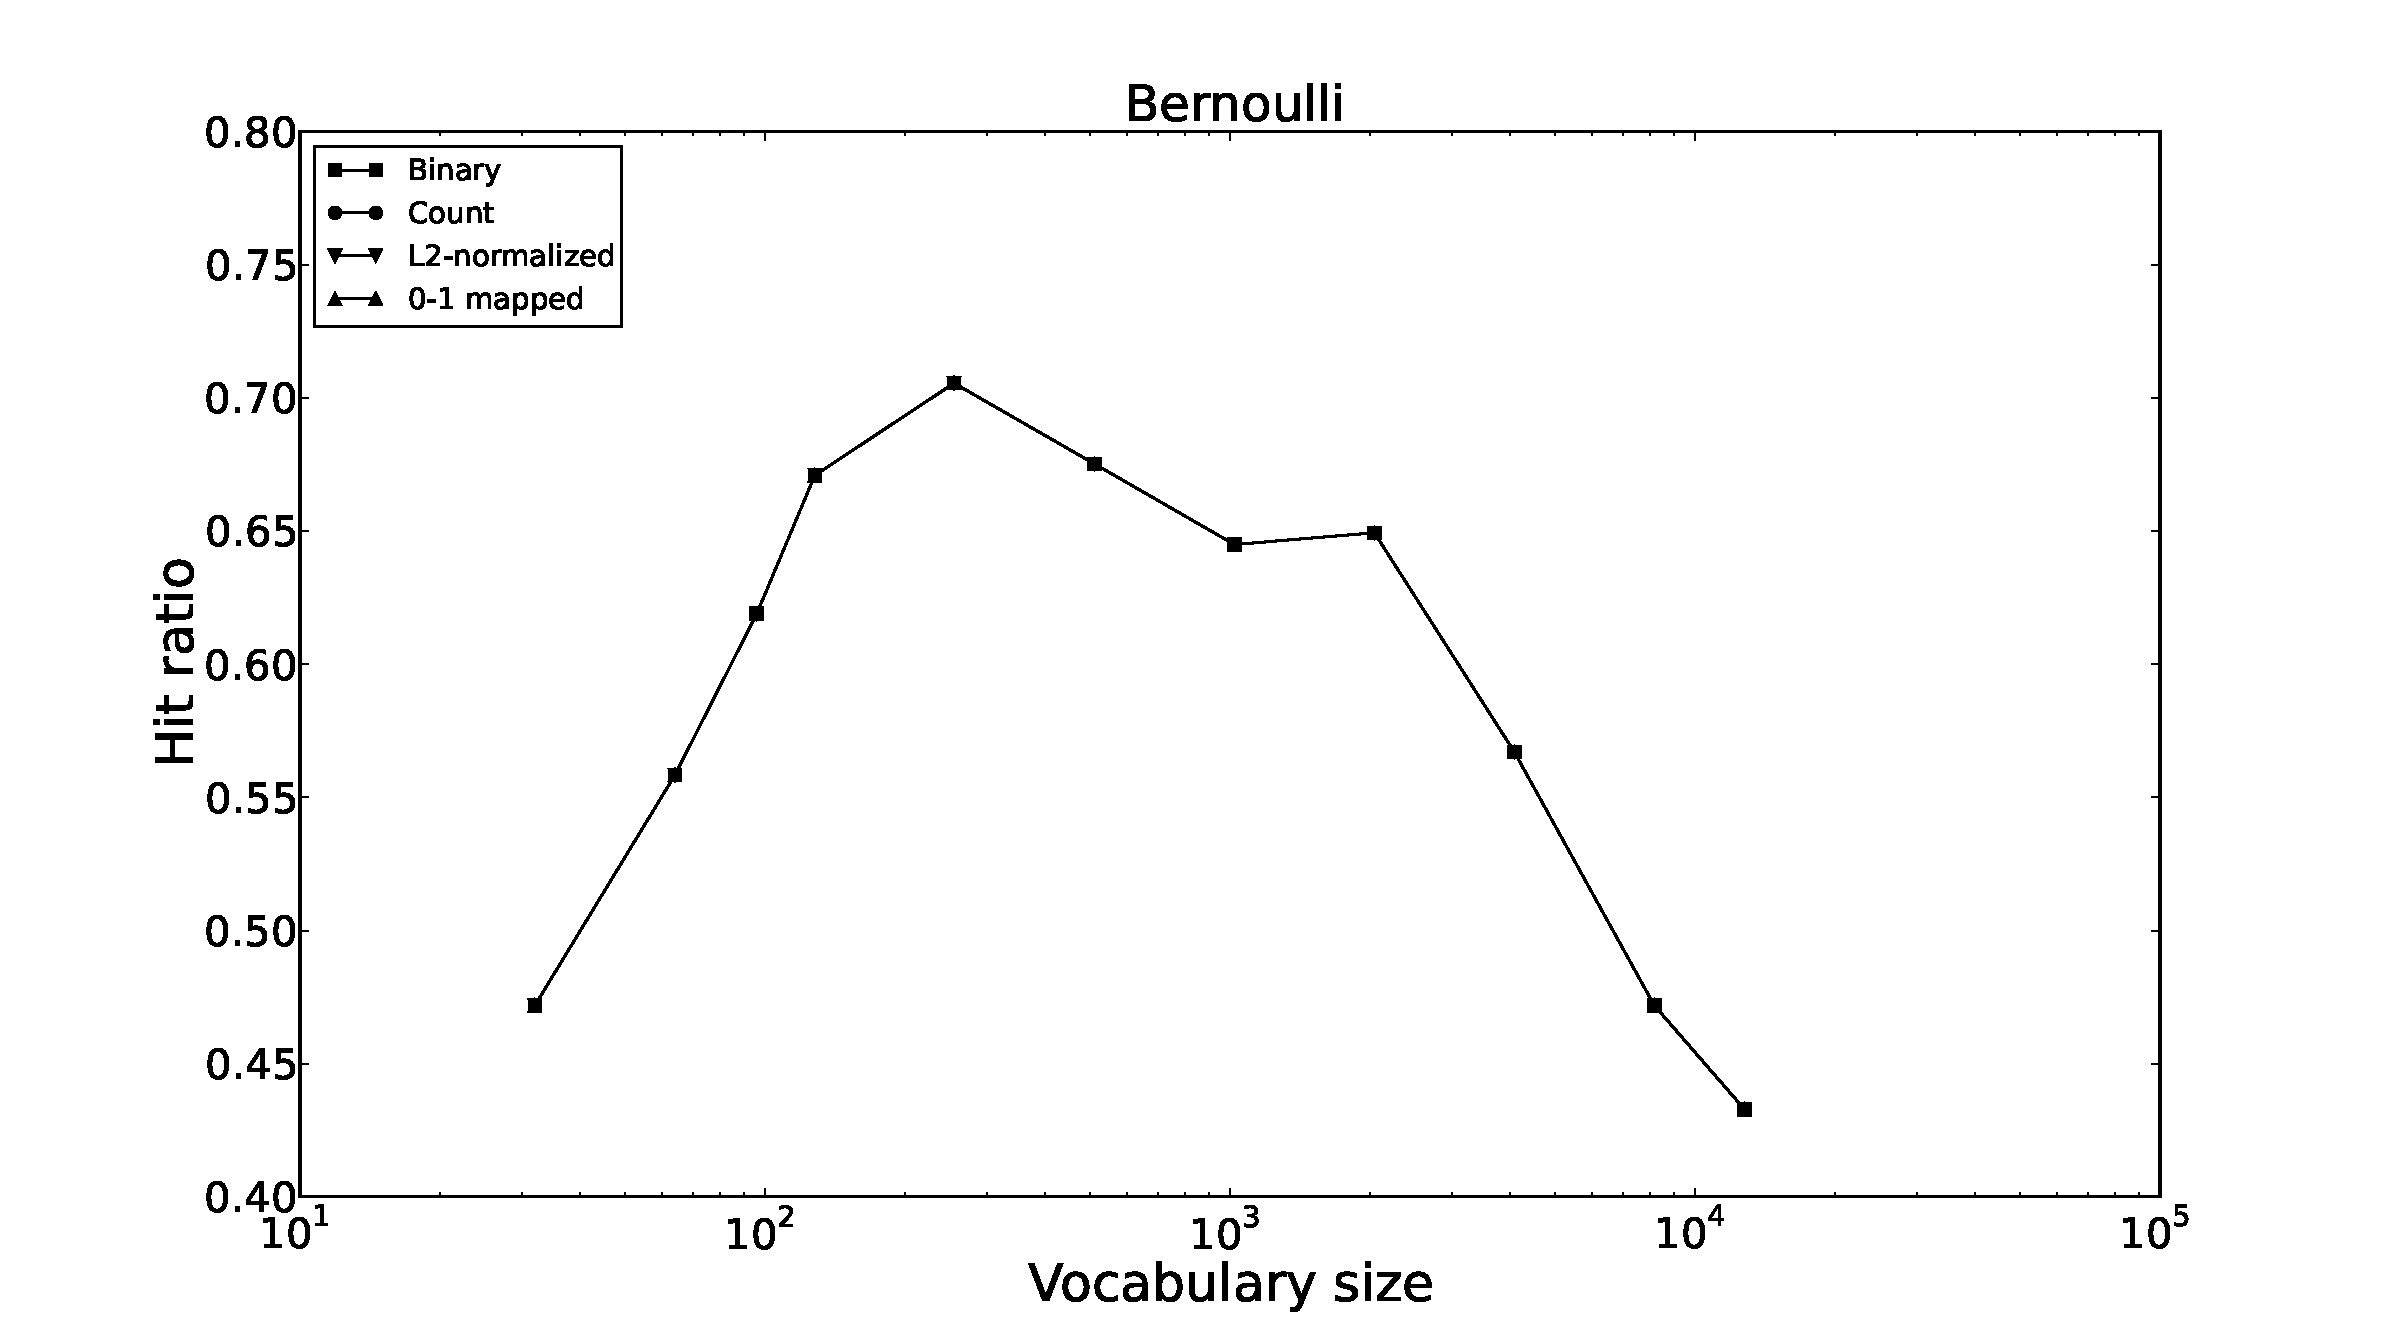
\includegraphics[width=\textwidth]{img/Bernoulli-hitrate-eps-converted-to.pdf}
		\caption{Hit ratio of Bernoulli classifier with varying vocabulary size. All values greater than zero is mapped to one, hence the different data types result in same accuracy.}
		\label{fig:hitratio-nb}
	\end{subfigure}
	~
	\begin{subfigure}[b]{\figwidth}
		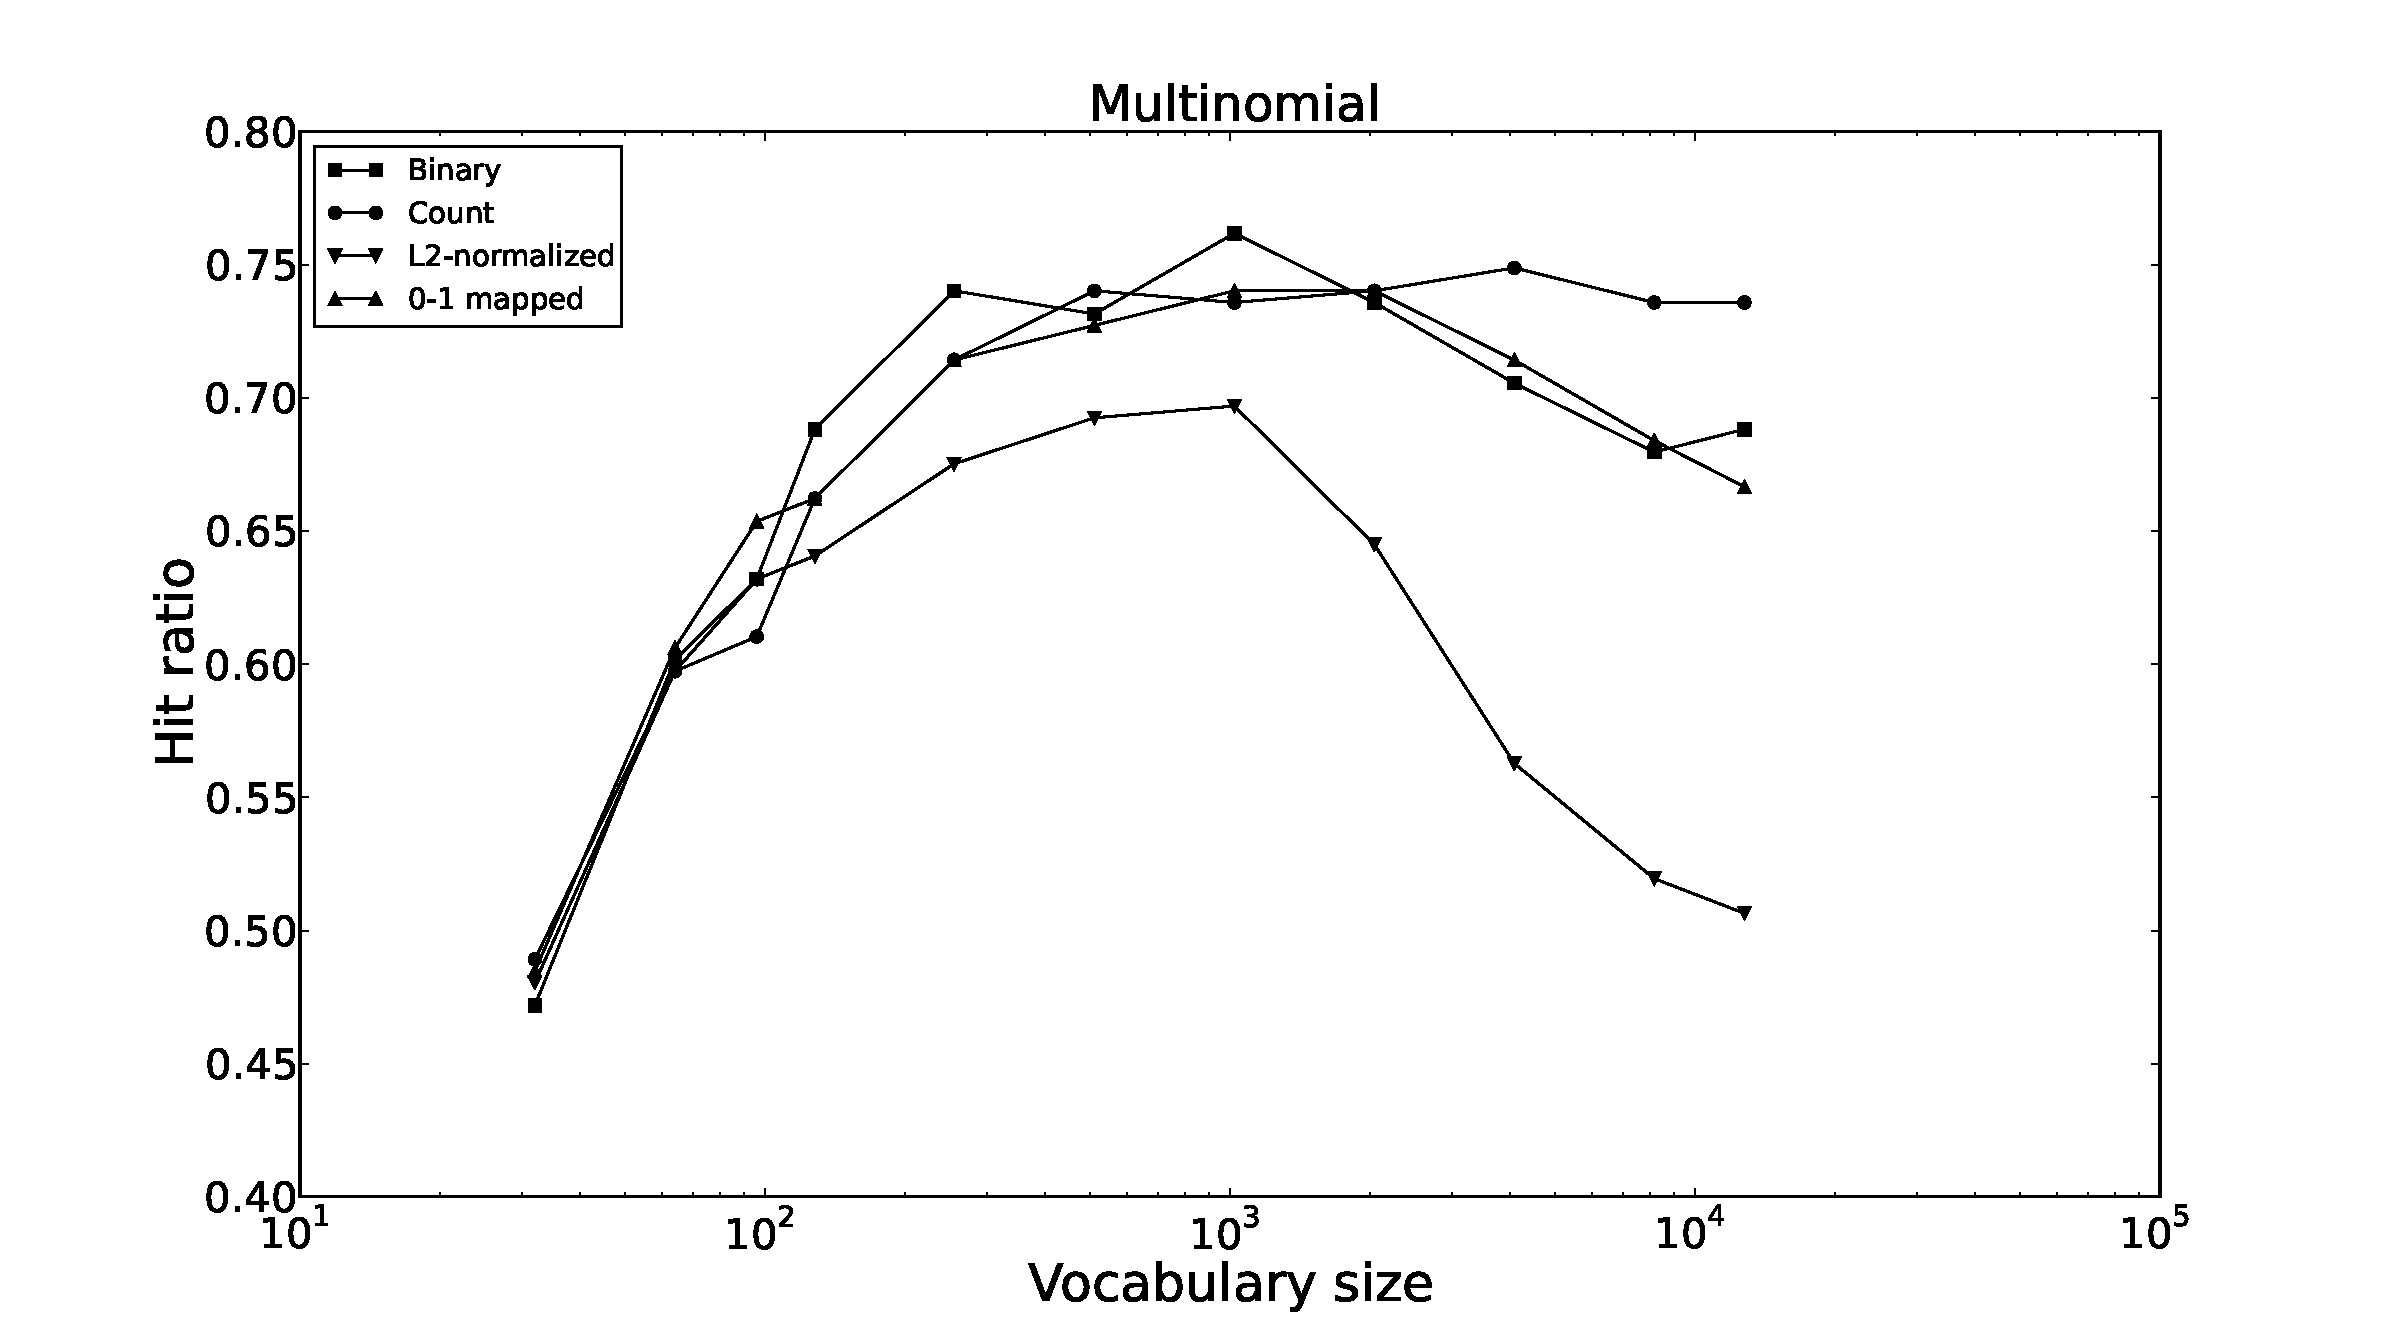
\includegraphics[width=\textwidth]{img/Multinomial-hitrate-eps-converted-to.pdf}
		\caption{Hit ratio of Multinomial classifier with varying vocabulary size.}
		\label{fig:hitratio-mn}
	\end{subfigure}
	\\
	\begin{subfigure}[b]{\figwidth}
		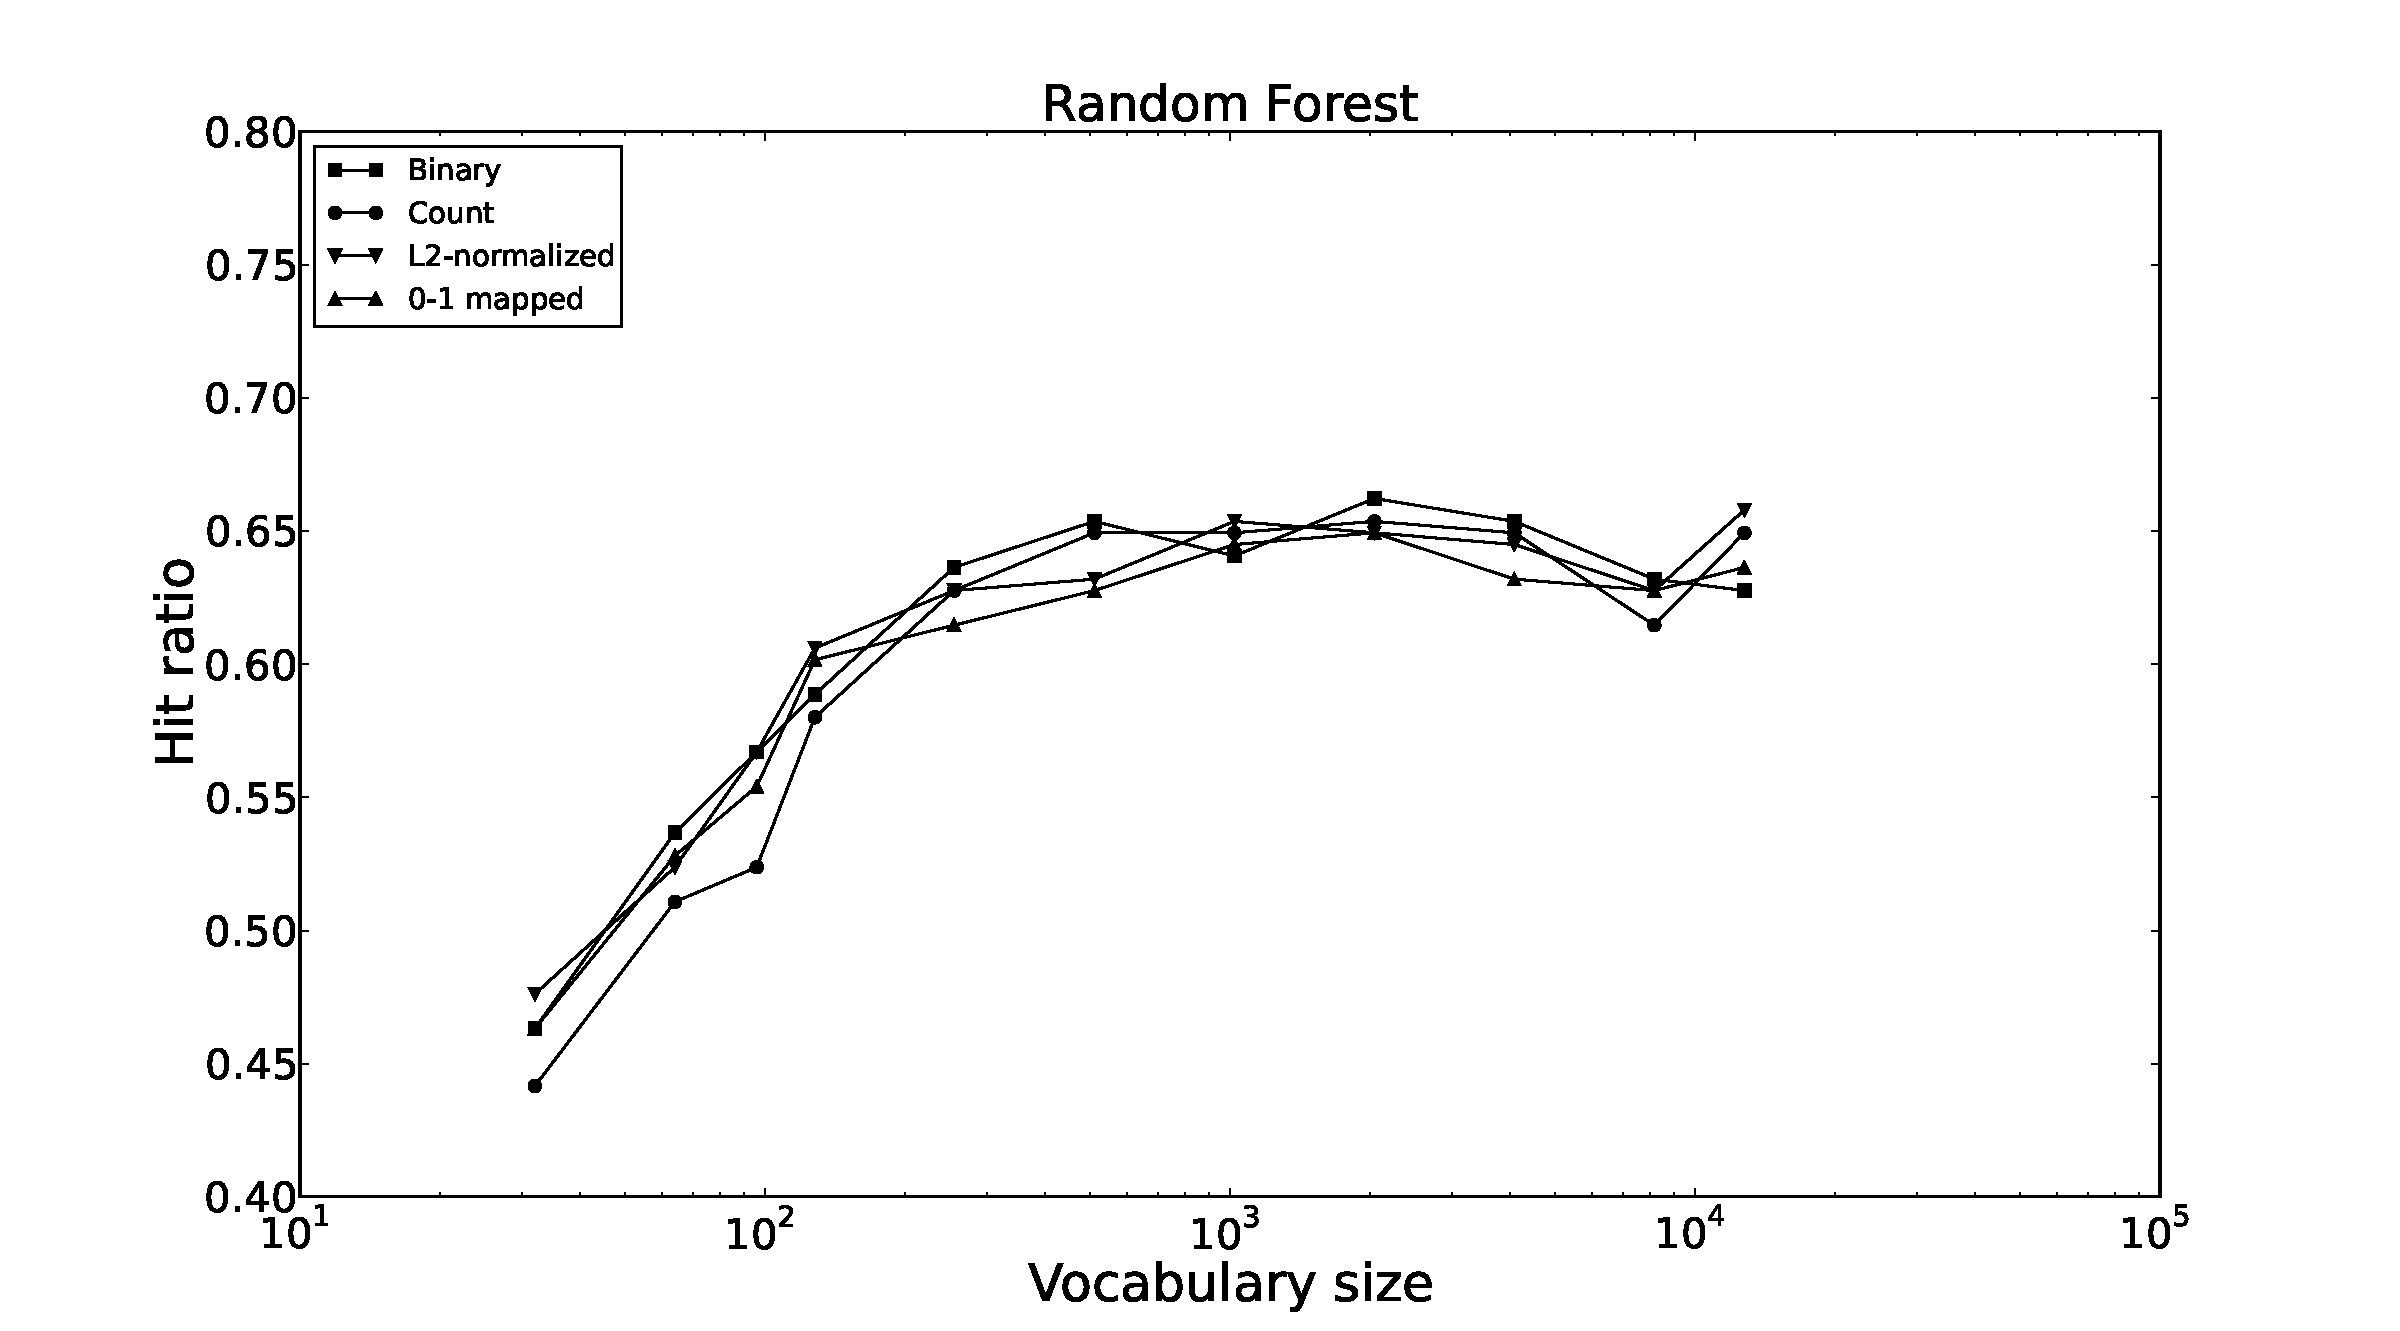
\includegraphics[width=\textwidth]{img/Random-Forest-hitrate-eps-converted-to.pdf}
		\caption{Hit ratio of Random Forest classifier with varying vocabulary size.}
		\label{fig:hitratio-rf}
	\end{subfigure}
	~
	\begin{subfigure}[b]{\figwidth}
		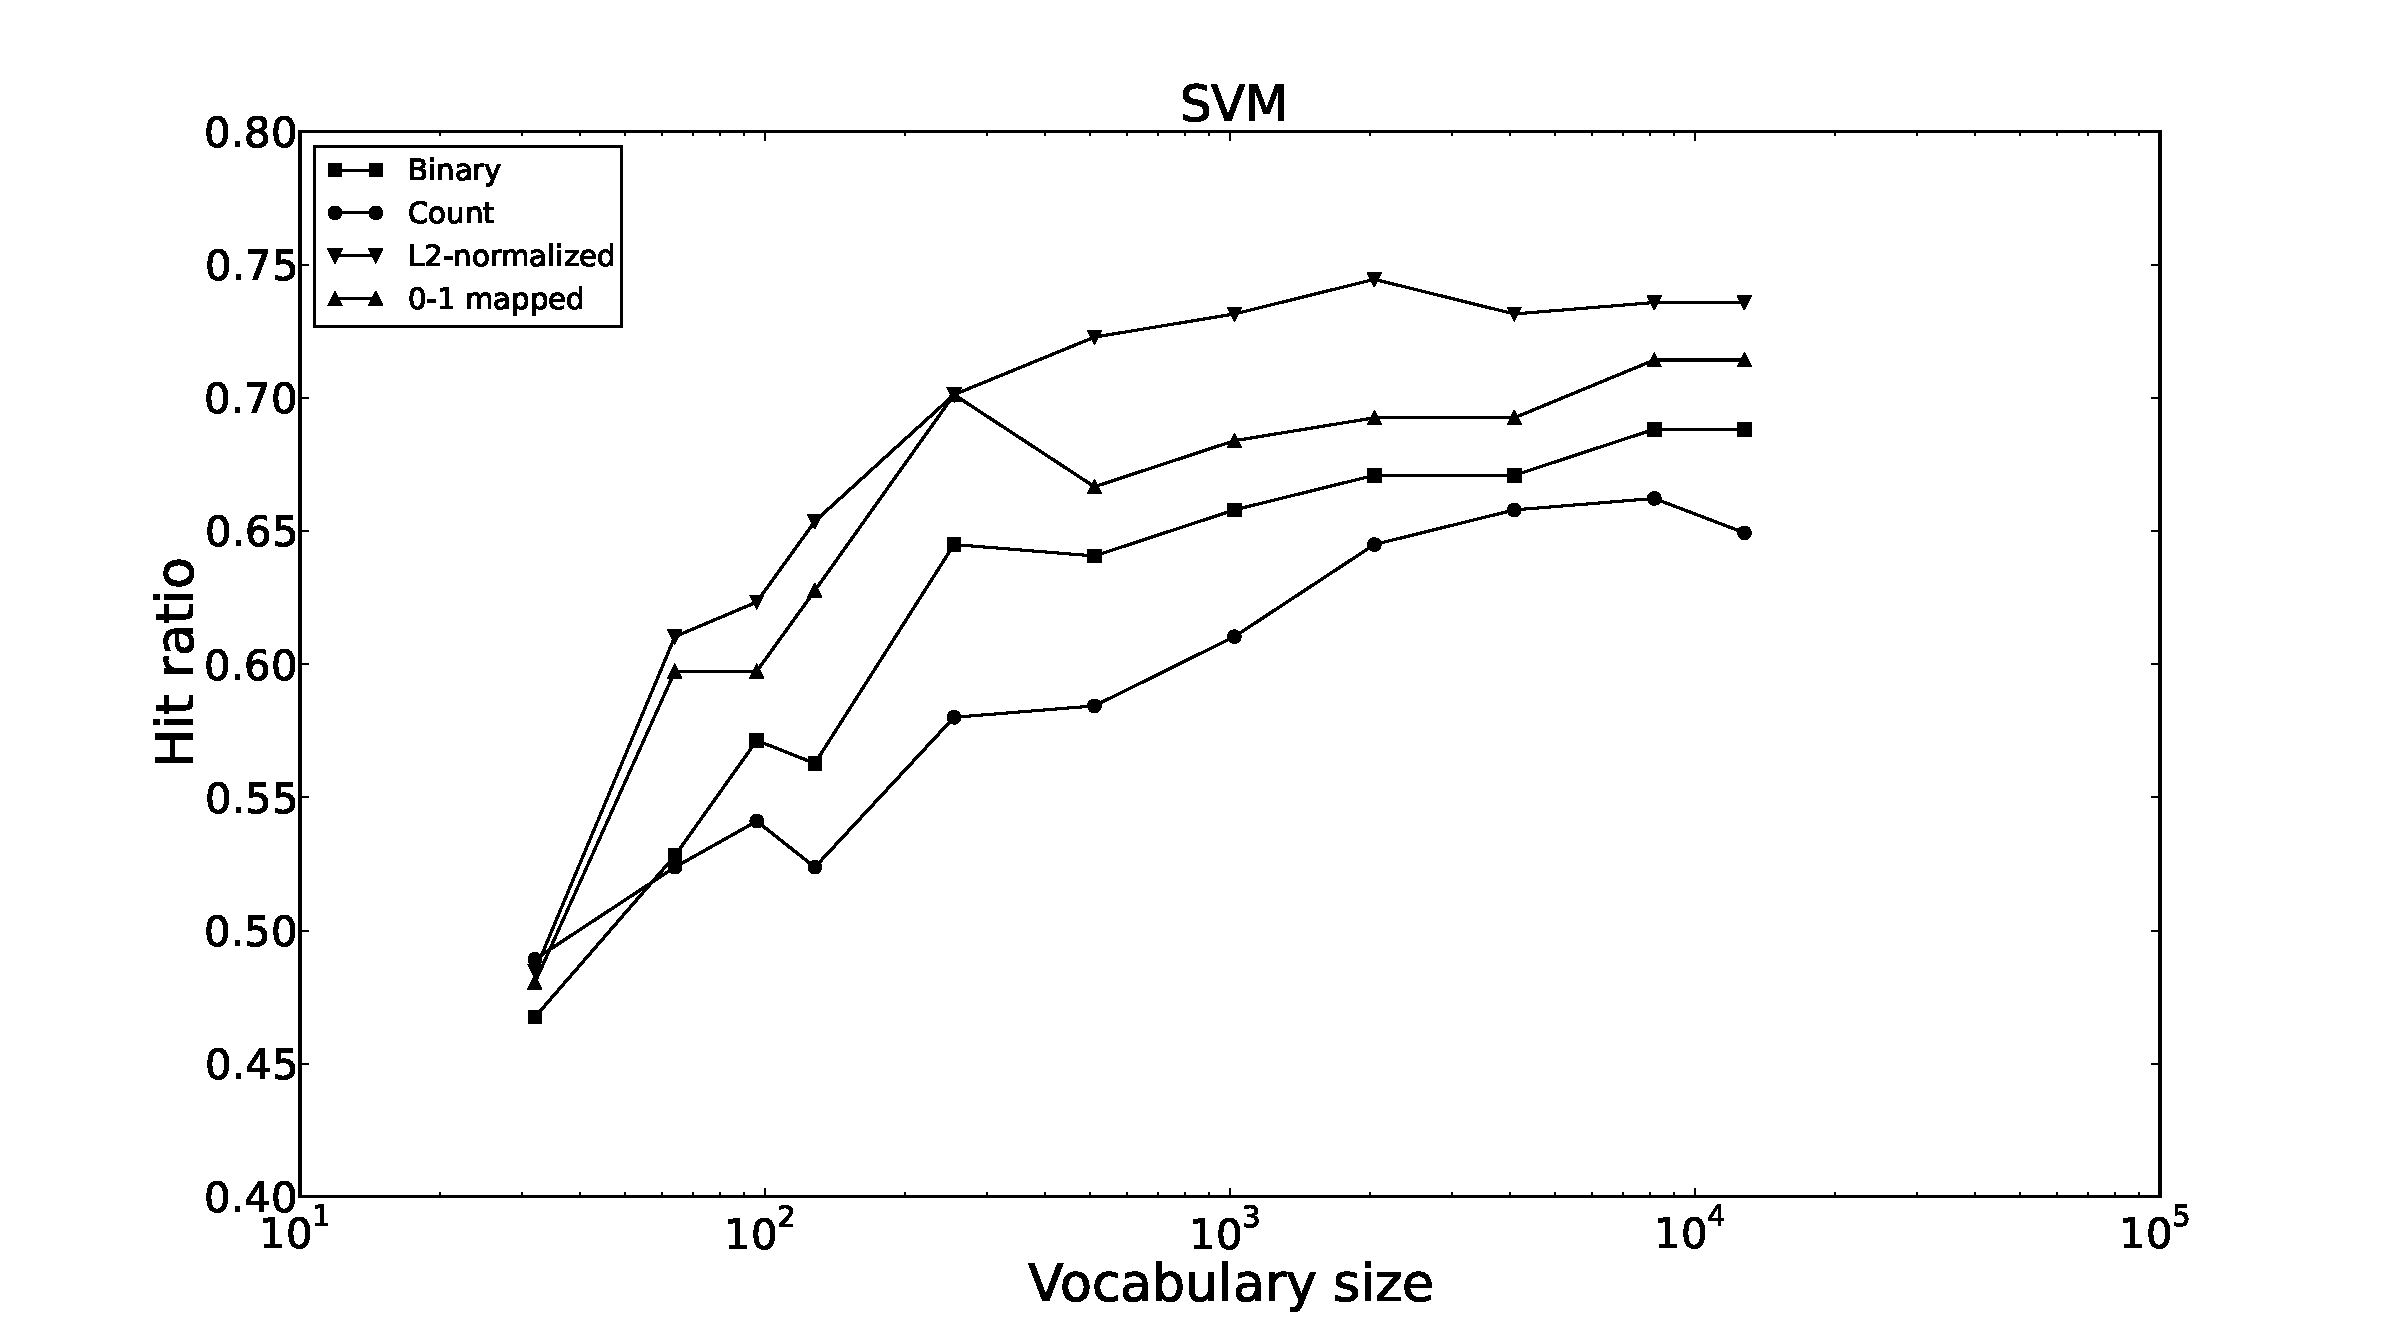
\includegraphics[width=\textwidth]{img/SVM-hitrate-eps-converted-to.pdf}
		\caption{Hit ratio of SVM classifier with varying vocabulary size.}
		\label{fig:hitratio-svm}
	\end{subfigure}
	\\
	\begin{subfigure}[b]{\figwidth}
		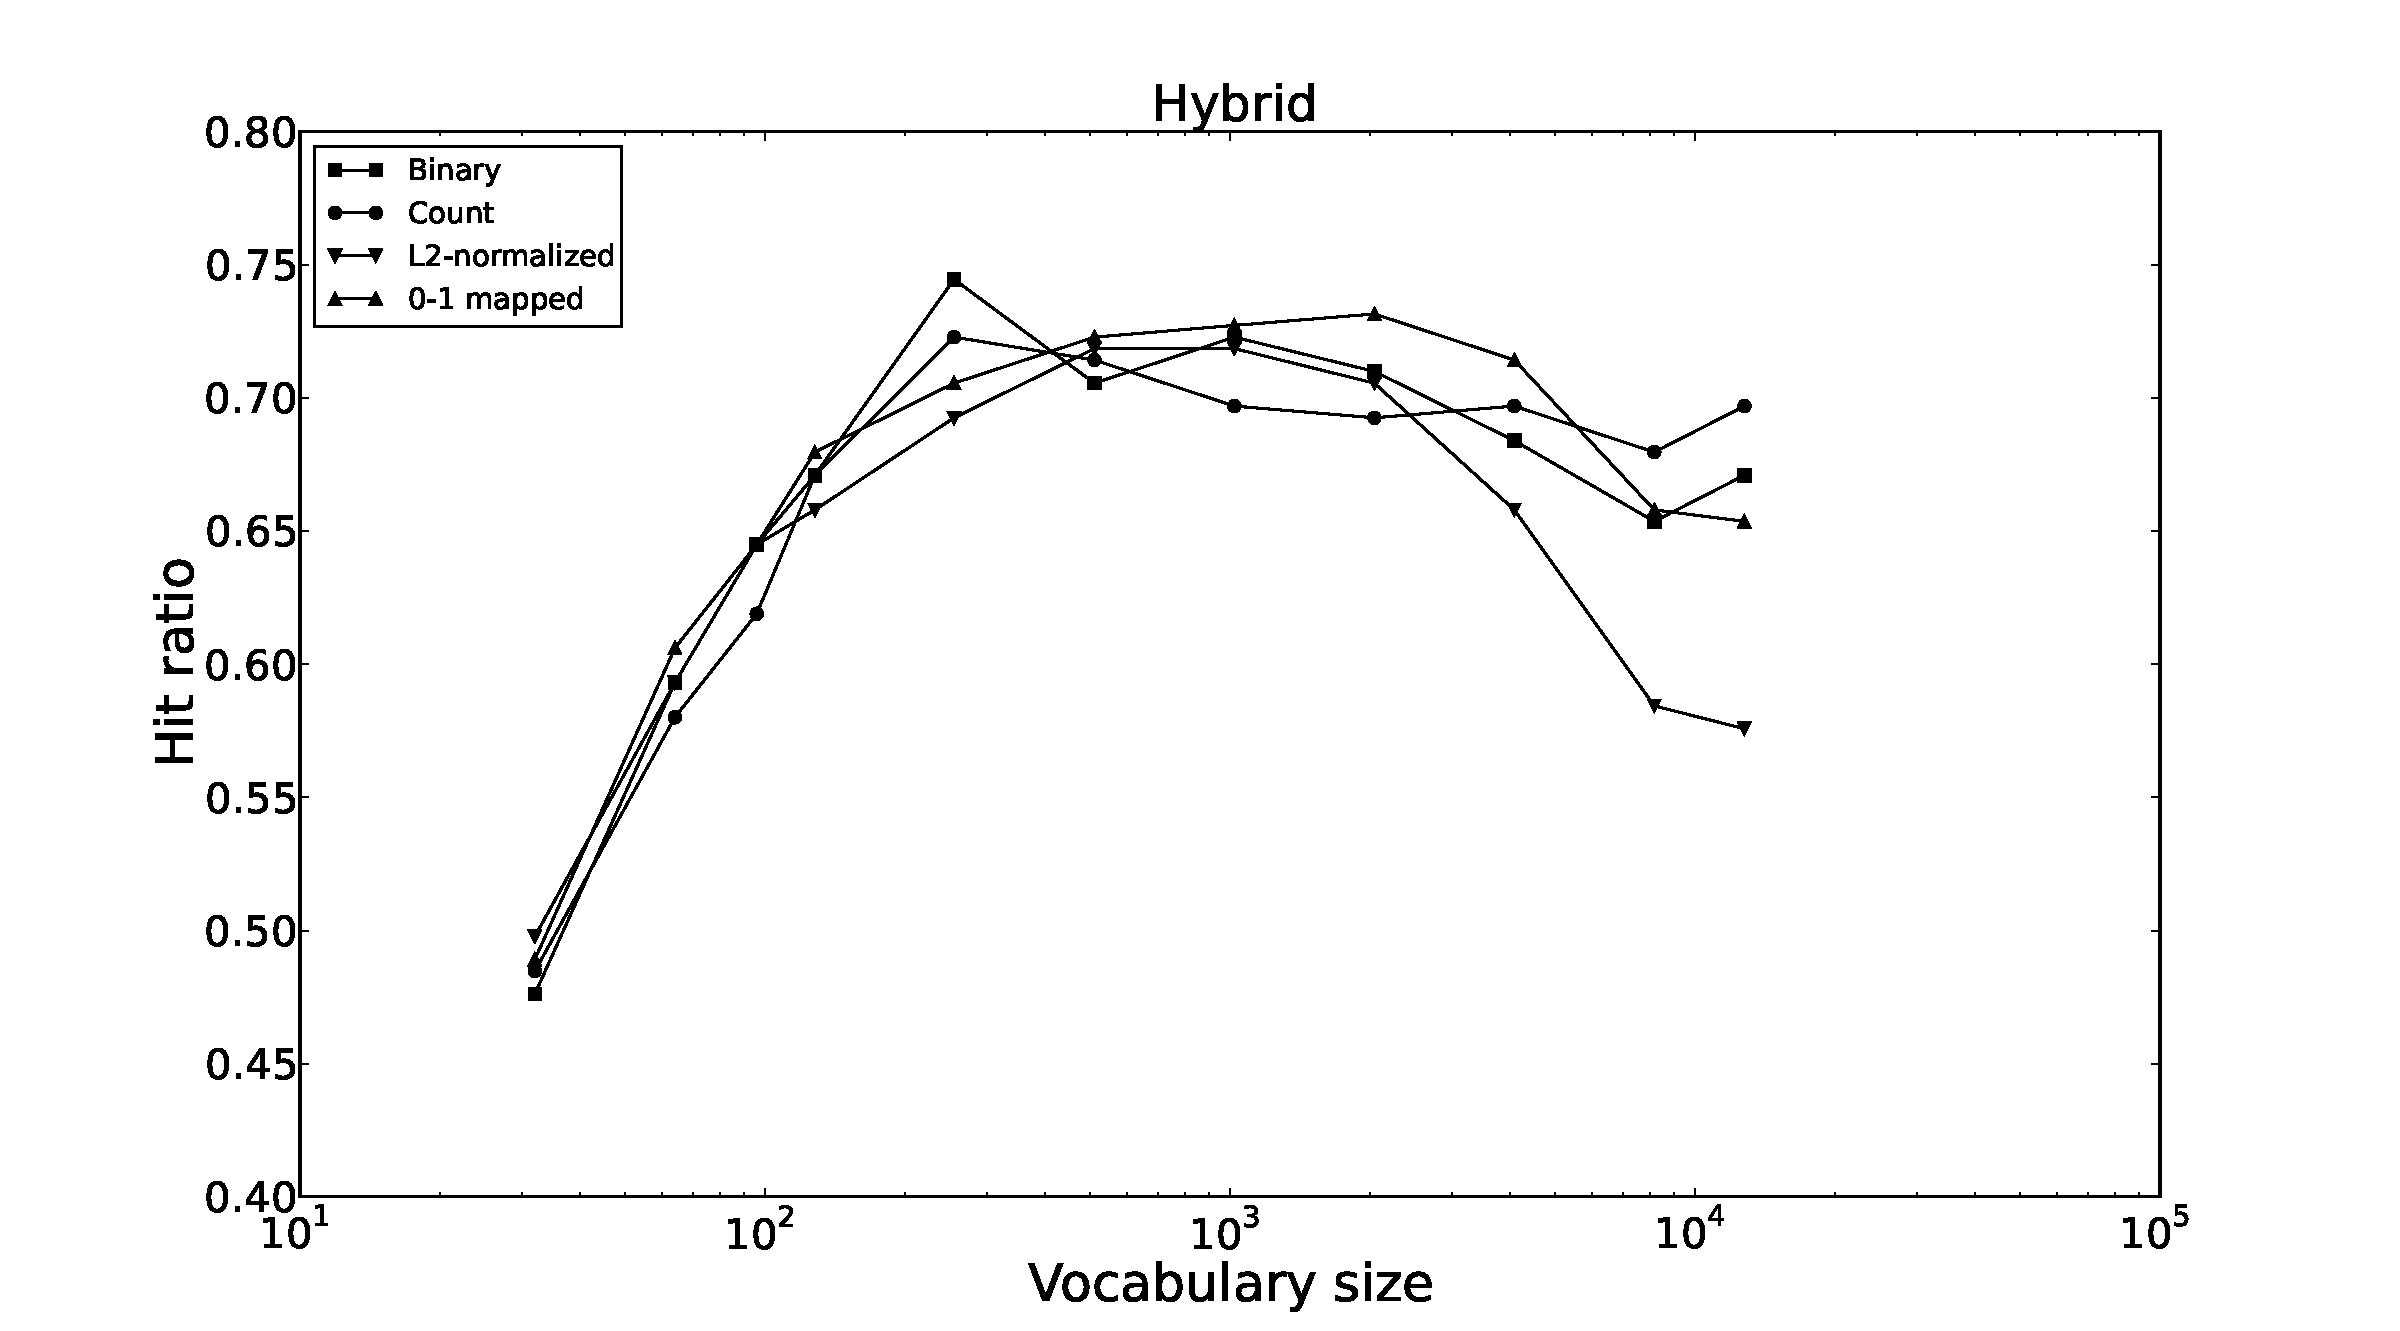
\includegraphics[width=\textwidth]{img/Hybrid-hitrate-eps-converted-to.pdf}
		\caption{Hit ratio of Hybrid classifier with varying vocabulary size.}
		\label{fig:hitratio-hybrid}
	\end{subfigure}
	\caption{Hit ratio vs vocabulary size}
	\label{fig:hitratio}
\end{figure}


\onecolumn
\renewcommand{\figwidth}{0.43\textwidth}
\begin{figure}[H]
	\centering
	\begin{subfigure}[b]{\figwidth}
		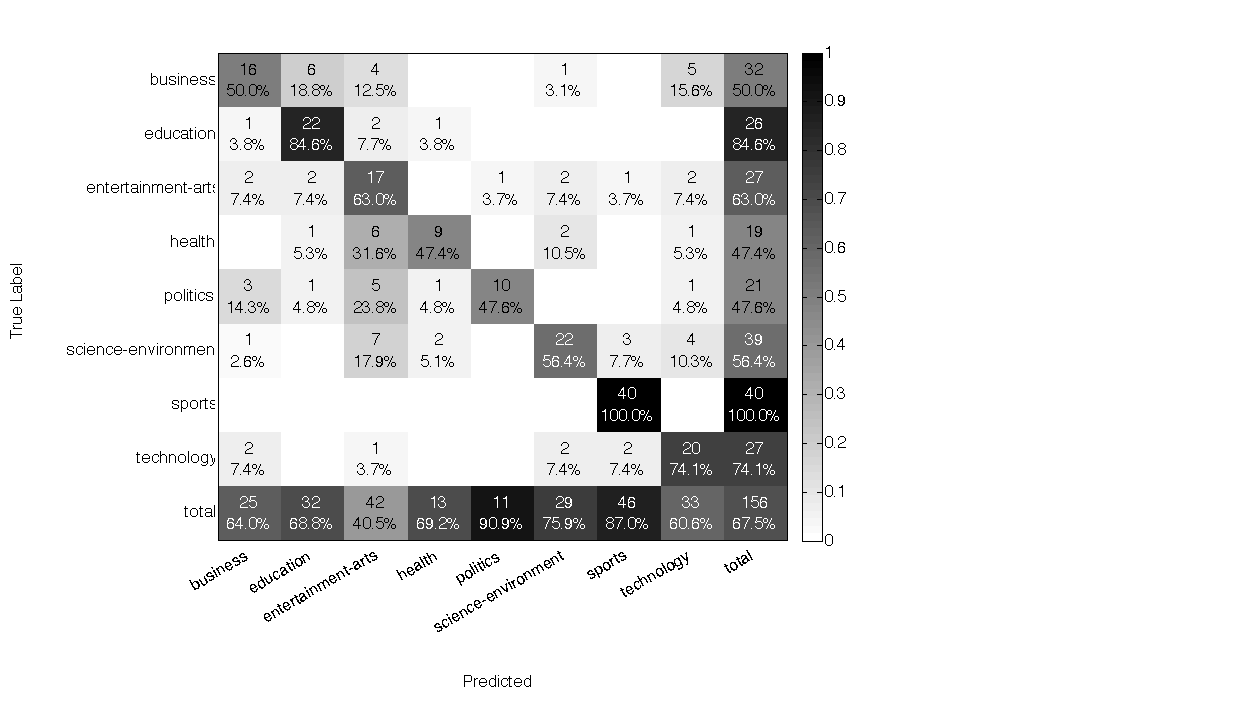
\includegraphics[width=\textwidth,trim=0 0 350 0, clip]{img/Bernou_percentile_5_count.png}
		\caption{Confusion matrix of Bernoulli.}
		\label{fig:confmat-be}
	\end{subfigure}
	~
	\begin{subfigure}[b]{\figwidth}
		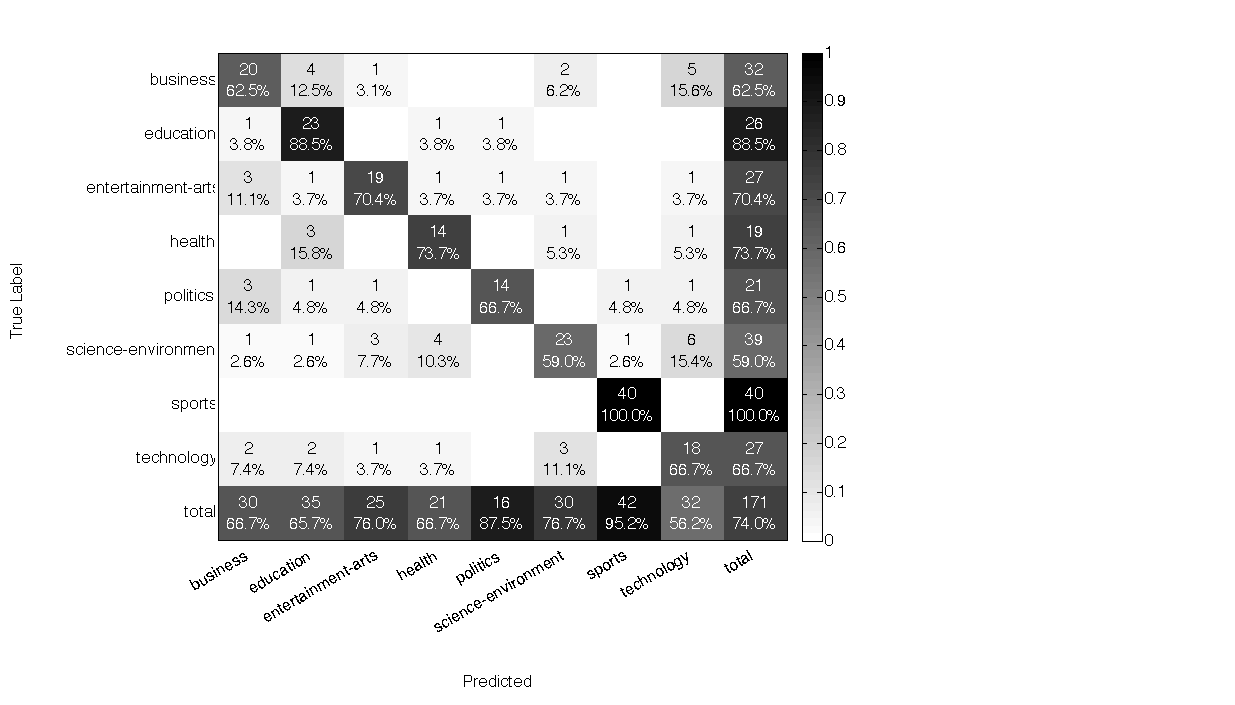
\includegraphics[width=\textwidth,trim=0 0 350 0, clip]{img/Multinomial_percentile_5_count.png}
		\caption{Confusion matrix of Multinomial.}
		\label{fig:confmat-mn}
	\end{subfigure}
	\\
	\begin{subfigure}[b]{\figwidth}
		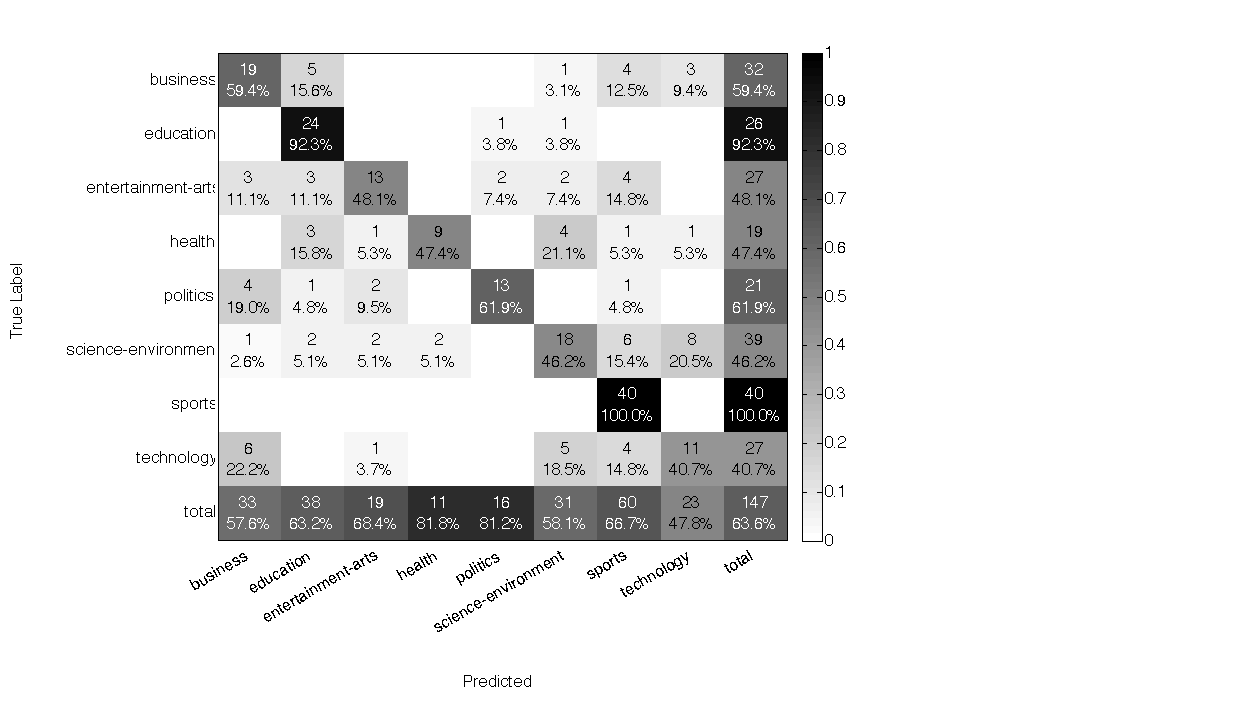
\includegraphics[width=\textwidth,trim=0 0 350 0, clip]{img/RandomForest_percentile_5_count.png}
		\caption{Confusion matrix of Random Forest.}
		\label{fig:confmat-rf}
	\end{subfigure}
	~
	\begin{subfigure}[b]{\figwidth}
		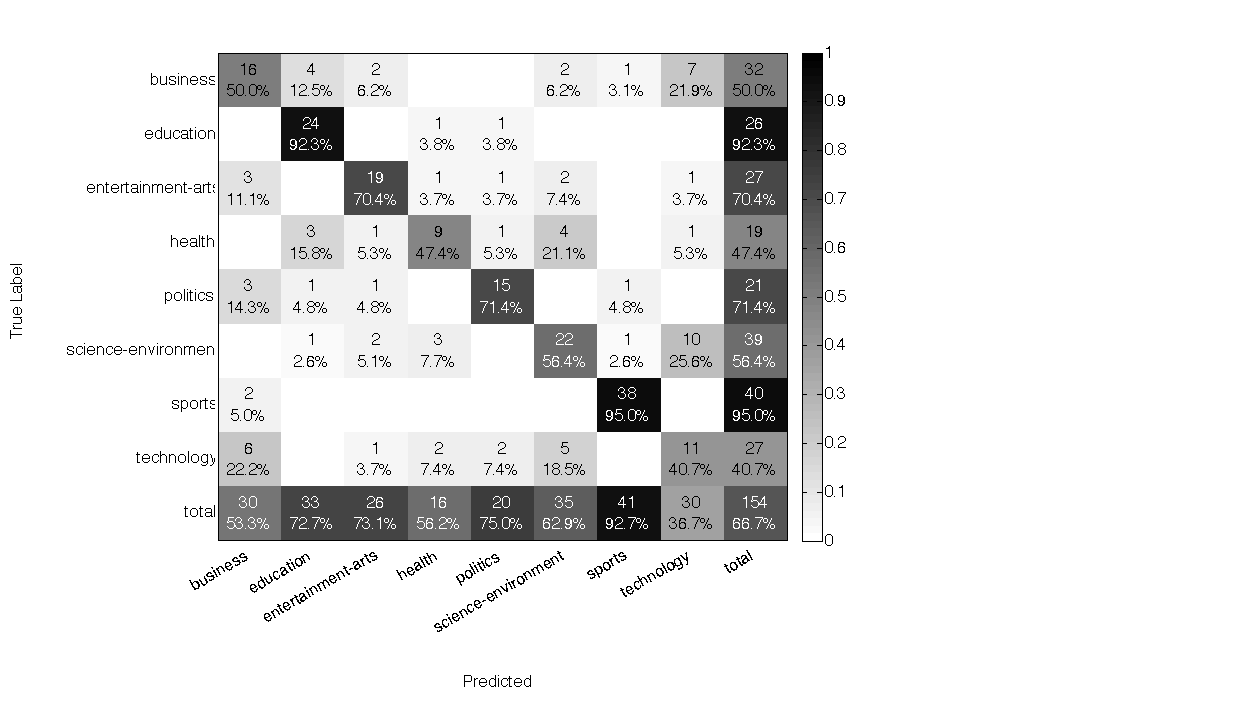
\includegraphics[width=\textwidth,trim=0 0 350 0, clip]{img/SVM_percentile_5_count.png}
		\caption{Confusion matrix of SVM.}
		\label{fig:confmat-svm}
	\end{subfigure}
	\\
	\begin{subfigure}[b]{\figwidth}
		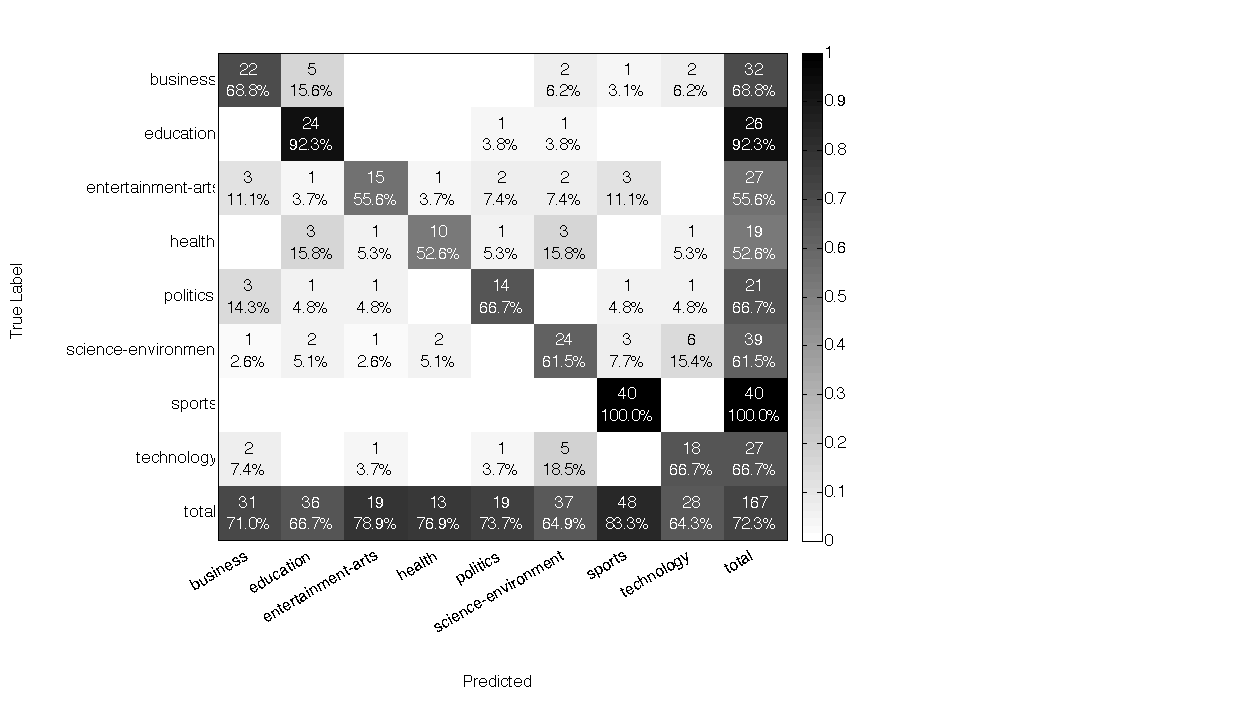
\includegraphics[width=\textwidth,trim=0 0 350 0, clip]{img/hybrid_percentile_5_count.png}
		\caption{Confusion matrix of Hybrid.}
		\label{fig:confmat-hybrid}
	\end{subfigure}
	\caption{Confusion matrices for the different classifiers. A total of 231 articles were tested. A vocabulary size of 511 words and the data type \emph{"Mapped value form 0 to 1"} were used.}
	\label{fig:confmat}
\end{figure}

\setlength\figureheight{0.25\linewidth}
\setlength\figurewidth{0.35\linewidth}
\begin{figure}[H]
	\centering
	\begin{subfigure}[b]{\figwidth}
		\tikzstyle{every node}=[font=\scriptsize]
		% This file was created by matlab2tikz v0.4.3.
% Copyright (c) 2008--2013, Nico Schlömer <nico.schloemer@gmail.com>
% All rights reserved.
% 
% The latest updates can be retrieved from
%   http://www.mathworks.com/matlabcentral/fileexchange/22022-matlab2tikz
% where you can also make suggestions and rate matlab2tikz.
% 
\begin{tikzpicture}

\begin{axis}[%
width=\figurewidth,
height=\figureheight,
scale only axis,
xmin=0,
xmax=503,
xlabel={Number of articles in training data},
ymin=0.5,
ymax=0.8,
ylabel={Hit ratio},
title={Bernoulli}
]
\addplot [
color=black,
solid,
mark=square,
mark options={solid},
forget plot
]
table[row sep=crcr]{
6 0.5325\\
11 0.6147\\
16 0.632\\
21 0.6407\\
41 0.6537\\
81 0.6753\\
161 0.6797\\
322 0.671\\
503 0.671\\
};
\addplot [
color=black,
solid,
mark=o,
mark options={solid},
forget plot
]
table[row sep=crcr]{
6 0.5325\\
11 0.6147\\
16 0.632\\
21 0.6407\\
41 0.6537\\
81 0.6753\\
161 0.6797\\
322 0.671\\
503 0.671\\
};
\addplot [
color=black,
solid,
mark=triangle,
mark options={solid,,rotate=180},
forget plot
]
table[row sep=crcr]{
6 0.5325\\
11 0.6147\\
16 0.632\\
21 0.6407\\
41 0.6537\\
81 0.6753\\
161 0.6797\\
322 0.671\\
503 0.671\\
};
\addplot [
color=black,
solid,
mark=triangle,
mark options={solid},
forget plot
]
table[row sep=crcr]{
6 0.5325\\
11 0.6147\\
16 0.632\\
21 0.6407\\
41 0.6537\\
81 0.6753\\
161 0.6797\\
322 0.671\\
503 0.671\\
};
\end{axis}
\end{tikzpicture}%
		\caption{Hit ratio of Bernoulli classifier with varying number of articles in training data. All values greater than zero are mapped to one, hence the different data types result in the same accuracy.}
		\label{fig:hitratio-data-nb}
	\end{subfigure}
	~
	\begin{subfigure}[b]{\figwidth}
		\tikzstyle{every node}=[font=\scriptsize]
		% This file was created by matlab2tikz v0.4.3.
% Copyright (c) 2008--2013, Nico Schlömer <nico.schloemer@gmail.com>
% All rights reserved.
% 
% The latest updates can be retrieved from
%   http://www.mathworks.com/matlabcentral/fileexchange/22022-matlab2tikz
% where you can also make suggestions and rate matlab2tikz.
% 
\begin{tikzpicture}

\begin{axis}[%
width=\figurewidth,
height=\figureheight,
scale only axis,
xmin=0,
xmax=503,
xlabel={Number of articles in training data},
ymin=0.5,
ymax=0.8,
ylabel={Hit ratio},
title={Multinomial}
]
\addplot [
color=black,
solid,
mark=square,
mark options={solid},
forget plot
]
table[row sep=crcr]{
6 0.6667\\
11 0.7186\\
16 0.7316\\
21 0.7316\\
41 0.7446\\
81 0.7532\\
161 0.7706\\
322 0.7316\\
503 0.7229\\
};
\addplot [
color=black,
solid,
mark=o,
mark options={solid},
forget plot
]
table[row sep=crcr]{
6 0.6883\\
11 0.7013\\
16 0.7186\\
21 0.7273\\
41 0.7403\\
81 0.7186\\
161 0.7489\\
322 0.7359\\
503 0.7446\\
};
\addplot [
color=black,
solid,
mark=triangle,
mark options={solid,,rotate=180},
forget plot
]
table[row sep=crcr]{
6 0.5844\\
11 0.6407\\
16 0.6753\\
21 0.684\\
41 0.7013\\
81 0.6883\\
161 0.6883\\
322 0.6883\\
503 0.6926\\
};
\addplot [
color=black,
solid,
mark=triangle,
mark options={solid},
forget plot
]
table[row sep=crcr]{
6 0.645\\
11 0.6883\\
16 0.7359\\
21 0.7316\\
41 0.7489\\
81 0.7446\\
161 0.7359\\
322 0.7186\\
503 0.7273\\
};
\end{axis}
\end{tikzpicture}%
		\caption{Hit ratio of Multinomial classifier with varying number of articles in training data.\\\ \\\ }
		\label{fig:hitratio-data-mn}
	\end{subfigure}
	\\
	\begin{subfigure}[b]{\figwidth}
		\tikzstyle{every node}=[font=\scriptsize]
		% This file was created by matlab2tikz v0.4.3.
% Copyright (c) 2008--2013, Nico Schlömer <nico.schloemer@gmail.com>
% All rights reserved.
% 
% The latest updates can be retrieved from
%   http://www.mathworks.com/matlabcentral/fileexchange/22022-matlab2tikz
% where you can also make suggestions and rate matlab2tikz.
% 
\begin{tikzpicture}

\begin{axis}[%
width=\figurewidth,
height=\figureheight,
scale only axis,
xmin=0,
xmax=503,
xlabel={Number of articles in training data},
ymin=0.5,
ymax=0.8,
ylabel={Hit ratio},
title={Random Forest}
]
\addplot [
color=black,
solid,
mark=square,
mark options={solid},
forget plot
]
table[row sep=crcr]{
6 0.5281\\
11 0.5714\\
16 0.6017\\
21 0.619\\
41 0.6623\\
81 0.658\\
161 0.684\\
322 0.645\\
503 0.6494\\
};
\addplot [
color=black,
solid,
mark=o,
mark options={solid},
forget plot
]
table[row sep=crcr]{
6 0.5541\\
11 0.5887\\
16 0.6147\\
21 0.619\\
41 0.6623\\
81 0.6623\\
161 0.6537\\
322 0.6537\\
503 0.6364\\
};
\addplot [
color=black,
solid,
mark=triangle,
mark options={solid,,rotate=180},
forget plot
]
table[row sep=crcr]{
6 0.5368\\
11 0.5974\\
16 0.6234\\
21 0.6407\\
41 0.632\\
81 0.645\\
161 0.6364\\
322 0.6407\\
503 0.6277\\
};
\addplot [
color=black,
solid,
mark=triangle,
mark options={solid},
forget plot
]
table[row sep=crcr]{
6 0.5238\\
11 0.5931\\
16 0.6277\\
21 0.6234\\
41 0.6234\\
81 0.6537\\
161 0.645\\
322 0.6407\\
503 0.6407\\
};
\end{axis}
\end{tikzpicture}%
		\caption{Hit ratio of Random Forest classifier with varying number of articles in training data.}
		\label{fig:hitratio-data-rf}
	\end{subfigure}
	~
	\begin{subfigure}[b]{\figwidth}
		\tikzstyle{every node}=[font=\scriptsize]
		% This file was created by matlab2tikz v0.4.3.
% Copyright (c) 2008--2013, Nico Schlömer <nico.schloemer@gmail.com>
% All rights reserved.
% 
% The latest updates can be retrieved from
%   http://www.mathworks.com/matlabcentral/fileexchange/22022-matlab2tikz
% where you can also make suggestions and rate matlab2tikz.
% 
\begin{tikzpicture}

\begin{axis}[%
width=\figurewidth,
height=\figureheight,
scale only axis,
xmin=0,
xmax=503,
xlabel={Number of articles in training data},
ymin=0.5,
ymax=0.8,
ylabel={Hit ratio},
title={SVM}
]
\addplot [
color=black,
solid,
mark=square,
mark options={solid},
forget plot
]
table[row sep=crcr]{
6 0.5108\\
11 0.5238\\
16 0.6017\\
21 0.5801\\
41 0.6407\\
81 0.6667\\
161 0.6537\\
322 0.6407\\
503 0.6407\\
};
\addplot [
color=black,
solid,
mark=o,
mark options={solid},
forget plot
]
table[row sep=crcr]{
6 0.5065\\
11 0.5238\\
16 0.5887\\
21 0.6017\\
41 0.6234\\
81 0.5844\\
161 0.5584\\
322 0.5887\\
503 0.5758\\
};
\addplot [
color=black,
solid,
mark=triangle,
mark options={solid,,rotate=180},
forget plot
]
table[row sep=crcr]{
6 0.6407\\
11 0.6623\\
16 0.7273\\
21 0.7013\\
41 0.7186\\
81 0.7489\\
161 0.7532\\
322 0.7359\\
503 0.7273\\
};
\addplot [
color=black,
solid,
mark=triangle,
mark options={solid},
forget plot
]
table[row sep=crcr]{
6 0.6104\\
11 0.5974\\
16 0.658\\
21 0.6537\\
41 0.6797\\
81 0.671\\
161 0.6926\\
322 0.6667\\
503 0.6537\\
};
\end{axis}
\end{tikzpicture}%
		\caption{Hit ratio of SVM classifier with varying number of articles in training data.}
		\label{fig:hitratio-data-svm}
	\end{subfigure}
	\\
	\begin{subfigure}[b]{\figwidth}
		\tikzstyle{every node}=[font=\scriptsize]
		% This file was created by matlab2tikz v0.4.3.
% Copyright (c) 2008--2013, Nico Schlömer <nico.schloemer@gmail.com>
% All rights reserved.
% 
% The latest updates can be retrieved from
%   http://www.mathworks.com/matlabcentral/fileexchange/22022-matlab2tikz
% where you can also make suggestions and rate matlab2tikz.
% 
\begin{tikzpicture}

\begin{axis}[%
width=\figurewidth,
height=\figureheight,
scale only axis,
xmin=0,
xmax=503,
xlabel={Number of articles in training data},
ymin=0.5,
ymax=0.8,
ylabel={Hit ratio},
title={Hybrid},
legend style={at={(1.03,1)},anchor=north west,draw=black,fill=white,legend cell align=left}
]
\addplot [
color=black,
solid,
mark=square,
mark options={solid}
]
table[row sep=crcr]{
6 0.6234\\
11 0.6494\\
16 0.6883\\
21 0.7013\\
41 0.7056\\
81 0.7186\\
161 0.7273\\
322 0.7056\\
503 0.7013\\
};
\addlegendentry{Binary};

\addplot [
color=black,
solid,
mark=o,
mark options={solid}
]
table[row sep=crcr]{
6 0.6537\\
11 0.658\\
16 0.697\\
21 0.6926\\
41 0.7143\\
81 0.6883\\
161 0.71\\
322 0.7056\\
503 0.7273\\
};
\addlegendentry{Count};

\addplot [
color=black,
solid,
mark=triangle,
mark options={solid,,rotate=180}
]
table[row sep=crcr]{
6 0.5931\\
11 0.645\\
16 0.6926\\
21 0.697\\
41 0.7143\\
81 0.7229\\
161 0.7186\\
322 0.7186\\
503 0.7229\\
};
\addlegendentry{L2-normalized};

\addplot [
color=black,
solid,
mark=triangle,
mark options={solid}
]
table[row sep=crcr]{
6 0.619\\
11 0.6623\\
16 0.7143\\
21 0.7056\\
41 0.7143\\
81 0.7143\\
161 0.7316\\
322 0.7186\\
503 0.7273\\
};
\addlegendentry{0-1 mapped};

\end{axis}
\end{tikzpicture}%
		\caption{Hit ratio of Hybrid classifier with varying number of articles in training data.}
		\label{fig:hitratio-data-hybrid}
	\end{subfigure}
	\caption{Hit ratio as a function of number of articles in training data for different classifiers and data types at a constant vocabulary size of 500 features after $\chi^2$ selection.}
	\label{fig:hitratio-data}
\end{figure}
\twocolumn
